\documentclass[11pt,a4paper]{article}
\usepackage[utf8]{inputenc}
\usepackage[spanish,es-tabla]{babel}
\usepackage{amsmath,amssymb}
\usepackage{geometry}
\geometry{margin=2.5cm}
\usepackage{graphicx}
\usepackage{booktabs}
\usepackage{float}
\usepackage{hyperref}
\usepackage{xcolor}
\usepackage{microtype}
\usepackage{caption}
\usepackage{subcaption}

\hypersetup{
    colorlinks=true,
    linkcolor=blue!70!black,
    citecolor=blue!70!black,
    urlcolor=blue!70!black
}

\title{\textbf{Laboratorio 5: Minería de Textos y Clasificación de Tweets sobre Desastres Naturales}\\
\large Entrega Parcial: Avances de Exploración, Preprocesamiento y Modelado Preliminar}

\author{
    \textbf{Javier Eduardo España} (23204)\\
    \textbf{Angel Esteban Esquit} (23249)\\
    \textbf{Bryan Gabriel Aguilar} (23354)\\[0.5em]
    \textit{Departamento de Ciencias de la Computación, Universidad del Valle de Guatemala}\\
    \textit{CC3084 - Data Science}
}
\date{\today}

\begin{document}

\maketitle

\begin{abstract}
En el presente informe de avance se documentan los resultados iniciales del procesamiento de lenguaje natural y minería de texto sobre el conjunto de datos \textit{Natural Language Processing with Disaster Tweets} de Kaggle. Se detallan las dimensiones y características estructurales del dataset, el análisis exploratorio de datos (EDA), el comportamiento de atributos como palabras clave y ubicaciones, y la distribución de longitudes de texto. Adicionalmente, se describe la metodología de preprocesamiento, extracción de n-gramas y el diseño de la arquitectura preliminar de clasificación.
\end{abstract}

\section{Introducción}
La rápida proliferación de redes sociales, en particular plataformas de microblogging como X (anteriormente Twitter), ha transformado la comunicación en situaciones de emergencia. Durante eventos catastróficos (terremotos, inundaciones, incendios forestales), los usuarios publican testimonios en tiempo real que son de alto valor para agencias de respuesta y organizaciones de ayuda humanitaria.

No obstante, clasificar de manera automatizada si un tweet describe una emergencia real o utiliza lenguaje metafórico (por ejemplo, \textit{"The new album is fire"} o \textit{"I'm drowning in homework"}) representa un reto significativo en el Procesamiento de Lenguaje Natural (NLP). El objetivo fundamental de este laboratorio es construir un sistema de minería de texto y aprendizaje automático capaz de discriminar entre tweets que reportan desastres reales ($target = 1$) y aquellos que no ($target = 0$).

\section{Descripción del Conjunto de Datos y Análisis Exploratorio}
El conjunto de datos utilizado corresponde a la competencia oficial de Kaggle \textit{"Natural Language Processing with Disaster Tweets"}. Está compuesto por más de 10,800 observaciones distribuidas en conjuntos de entrenamiento (\texttt{train.csv}) y prueba (\texttt{test.csv}).

\subsection{Estructura de Variables}
El conjunto de entrenamiento contiene 7,613 filas y 5 columnas principales:
\begin{itemize}
    \item \textbf{id}: Identificador numérico único de cada tweet.
    \item \textbf{keyword}: Palabra clave relevante asociada al tweet (puede contener valores nulos).
    \item \textbf{location}: Ubicación geográfica declarada por el autor (texto libre, alta tasa de valores nulos).
    \item \textbf{text}: Contenido textual íntegro del tweet.
    \item \textbf{target}: Etiqueta binaria de clasificación donde 1 denota un desastre real y 0 denota no desastre.
\end{itemize}

\subsection{Distribución de Clases y Valores Faltantes}
La Figura~\ref{fig:target_missing} ilustra la distribución de la variable objetivo y el porcentaje de valores nulos en cada variable. De los 7,613 tweets de entrenamiento, 4,342 (57.0\%) corresponden a mensajes que no describen desastres, mientras que 3,271 (43.0\%) corresponden a emergencias reales. Se observa un ligero desbalance, pero la proporción es adecuada para entrenamiento sin requerir técnicas severas de submuestreo o sobremuestreo.

\begin{figure}[H]
    \centering
    \begin{subfigure}[b]{0.48\textwidth}
        \centering
        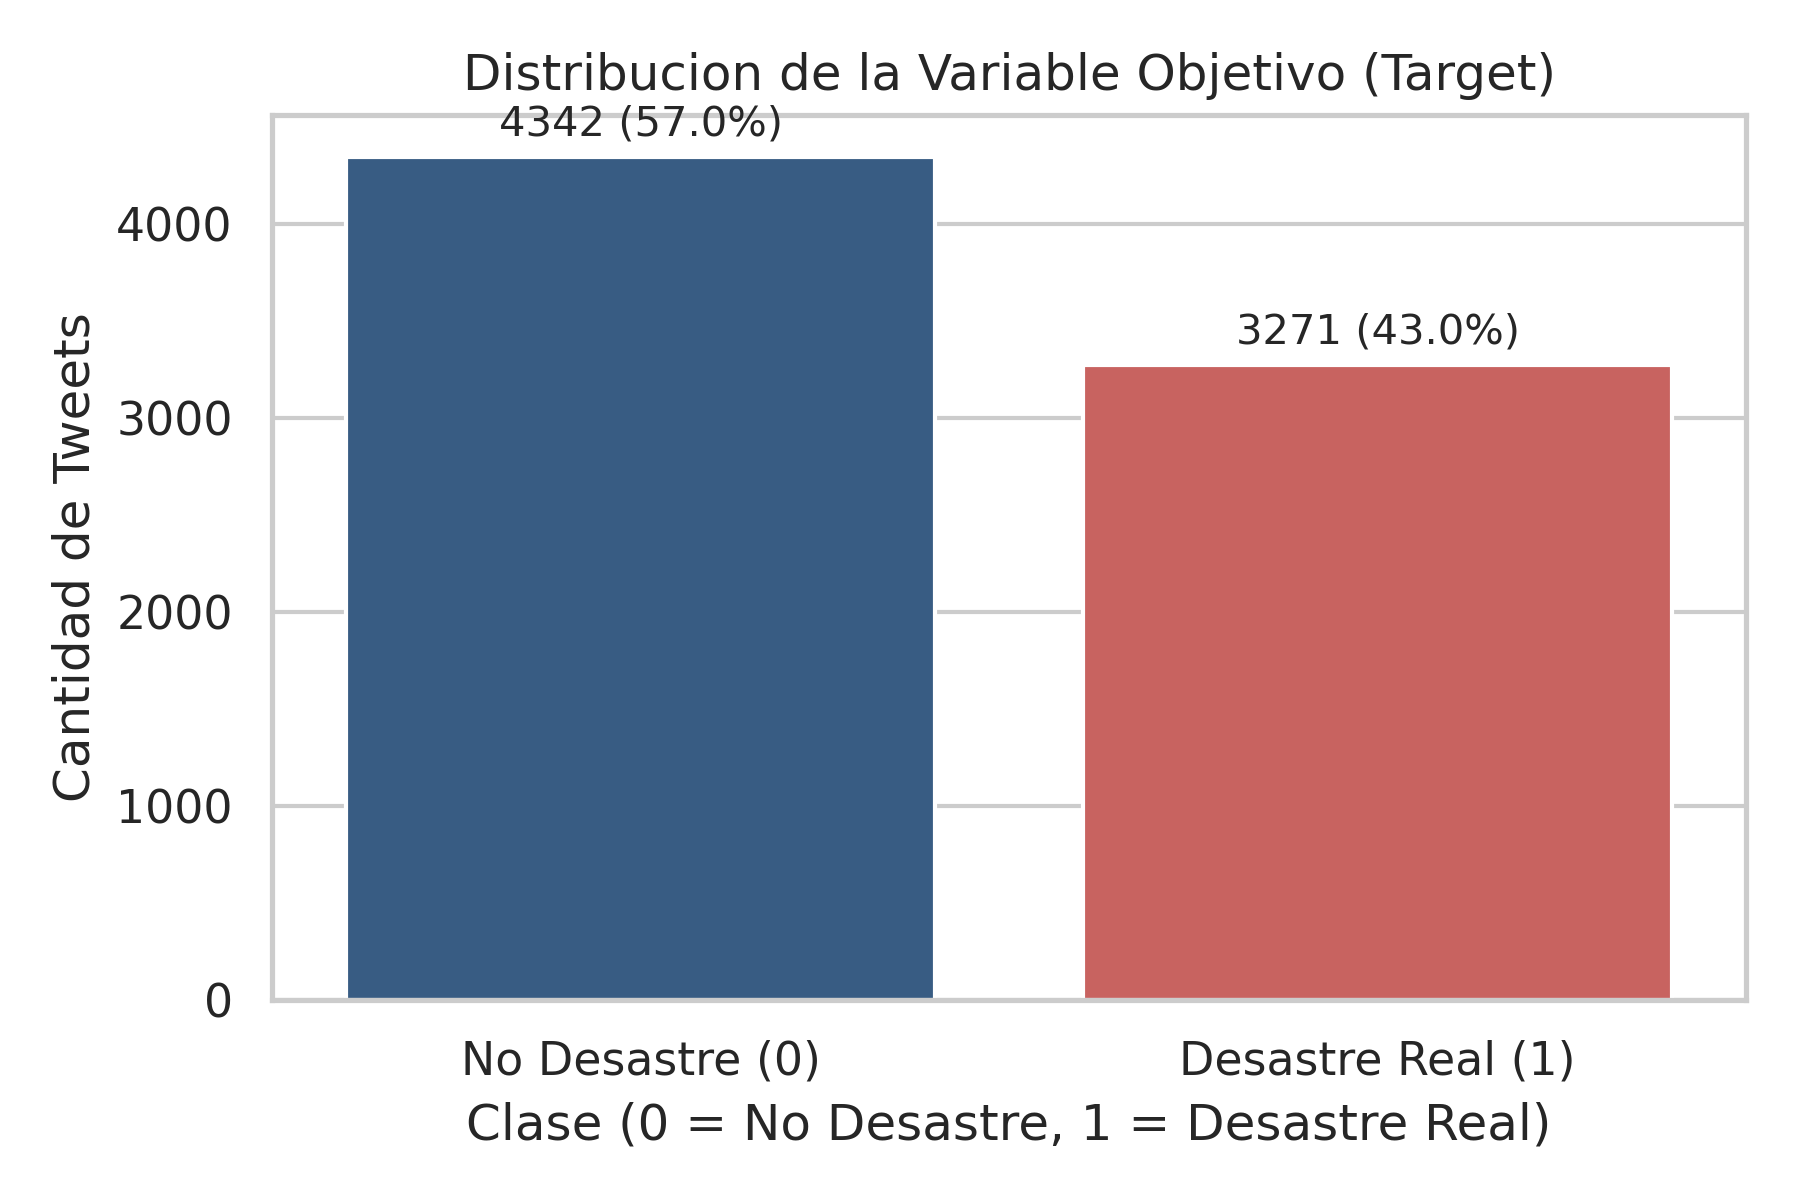
\includegraphics[width=\textwidth]{figures/target_distribution.png}
        \caption{Distribución de la variable objetivo.}
        \label{fig:target_dist}
    \end{subfigure}
    \hfill
    \begin{subfigure}[b]{0.48\textwidth}
        \centering
        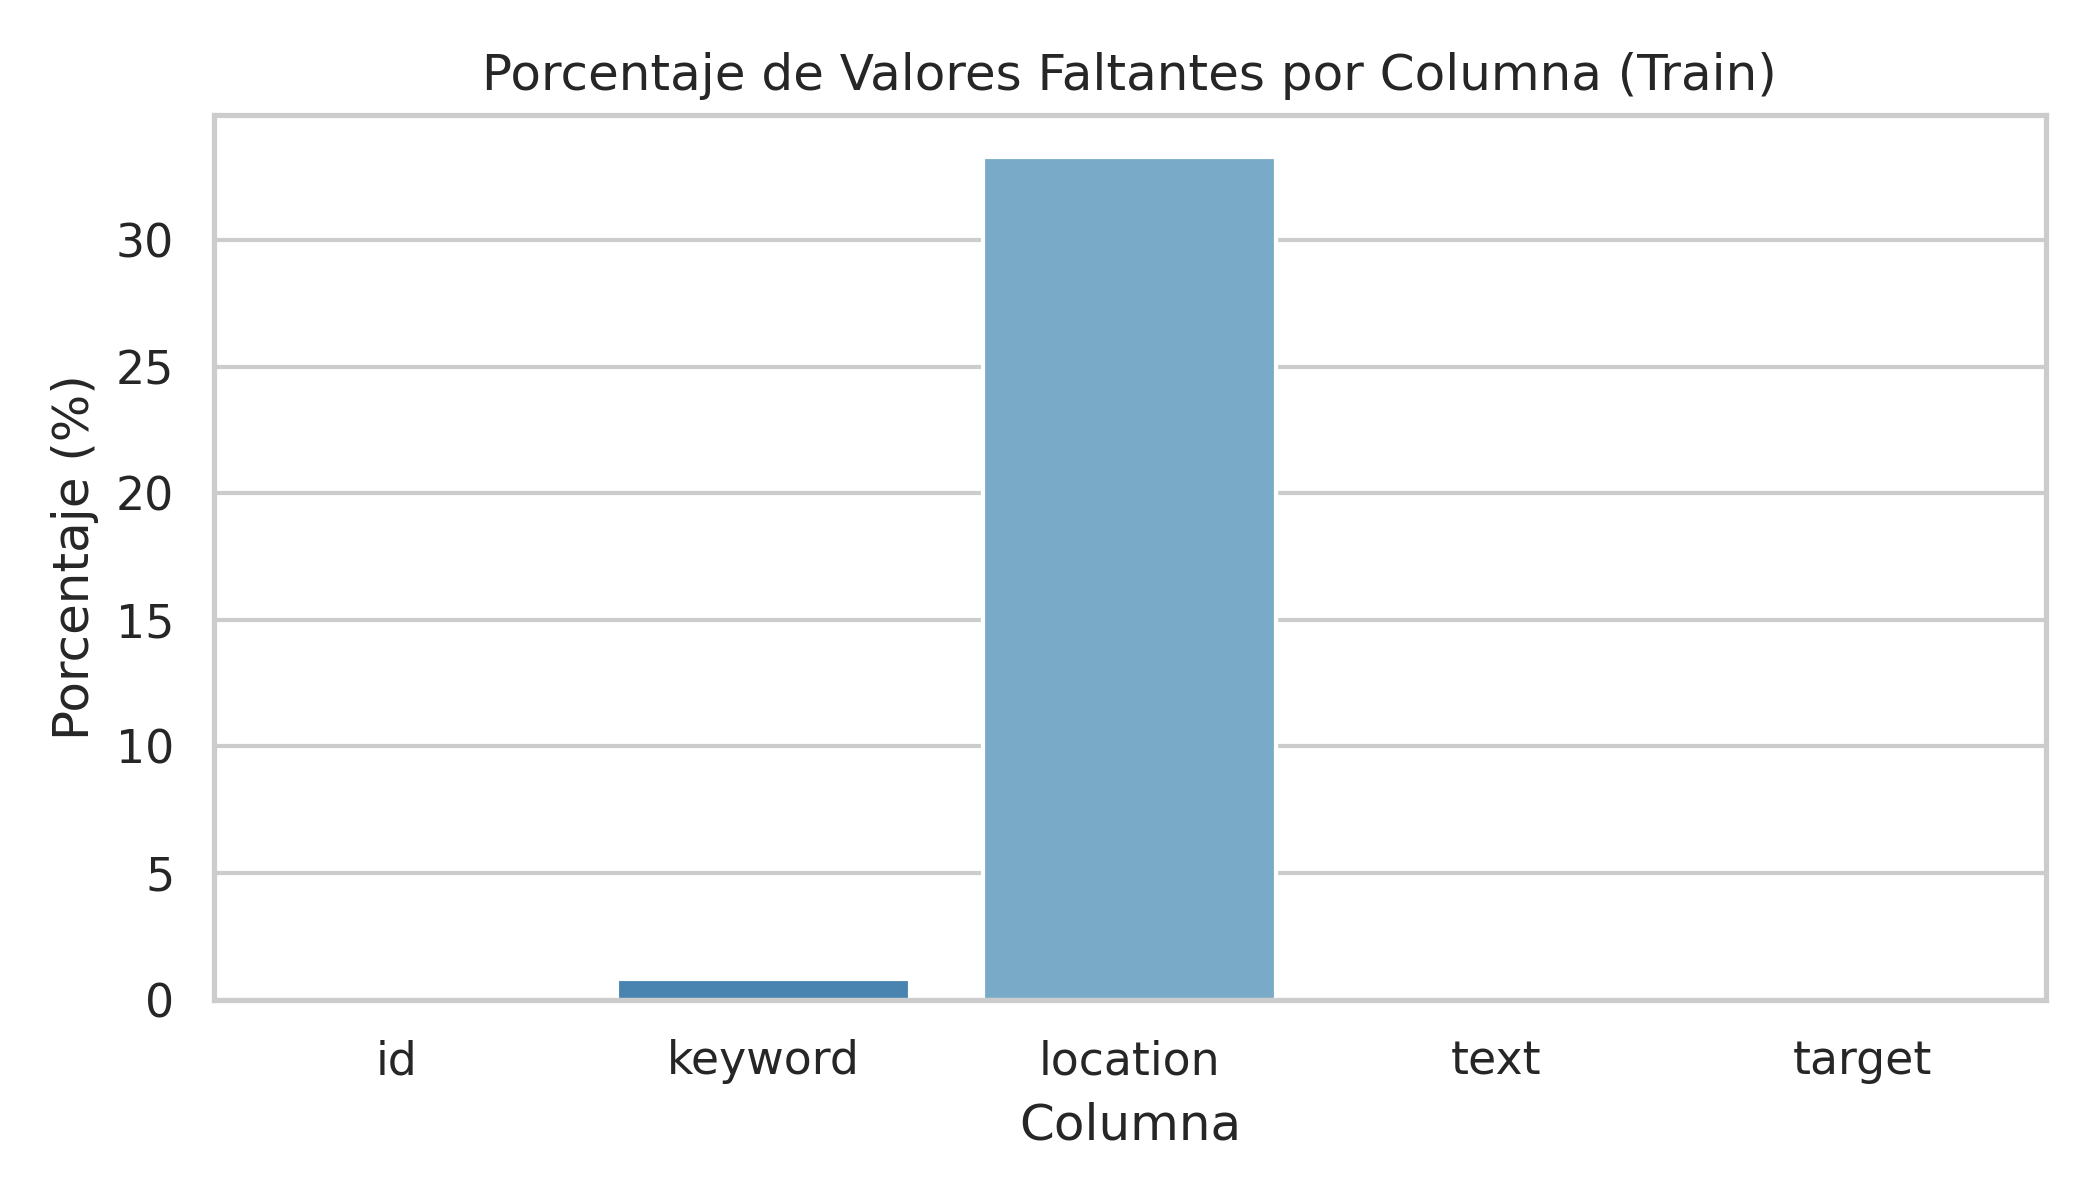
\includegraphics[width=\textwidth]{figures/missing_values.png}
        \caption{Porcentaje de valores faltantes por atributo.}
        \label{fig:missing_vals}
    \end{subfigure}
    \caption{Distribución de clases y valores faltantes en el conjunto de entrenamiento.}
    \label{fig:target_missing}
\end{figure}

Respecto a los valores nulos, la variable \texttt{location} presenta 2,533 valores faltantes (33.3\%), mientras que \texttt{keyword} contiene 61 nulos (0.8\%). La variable textual principal \texttt{text} y la variable objetivo \texttt{target} no contienen valores nulos.

\subsection{Análisis de Palabras Clave (Keywords) y Longitud de Texto}
El análisis de las palabras clave revela disparidades significativas entre clases. En la Figura~\ref{fig:top_keywords} se aprecian las palabras clave más frecuentes para cada clase. En tweets de desastres reales predominan términos técnicos y operacionales como \textit{derailment}, \textit{wreckage}, \textit{outbreak} y \textit{typhoon}. En contraste, en tweets de no desastre aparecen términos con connotación coloquial o figurativa como \textit{body\%20bags}, \textit{harm}, \textit{armageddon} y \textit{deluge}.

\begin{figure}[H]
    \centering
    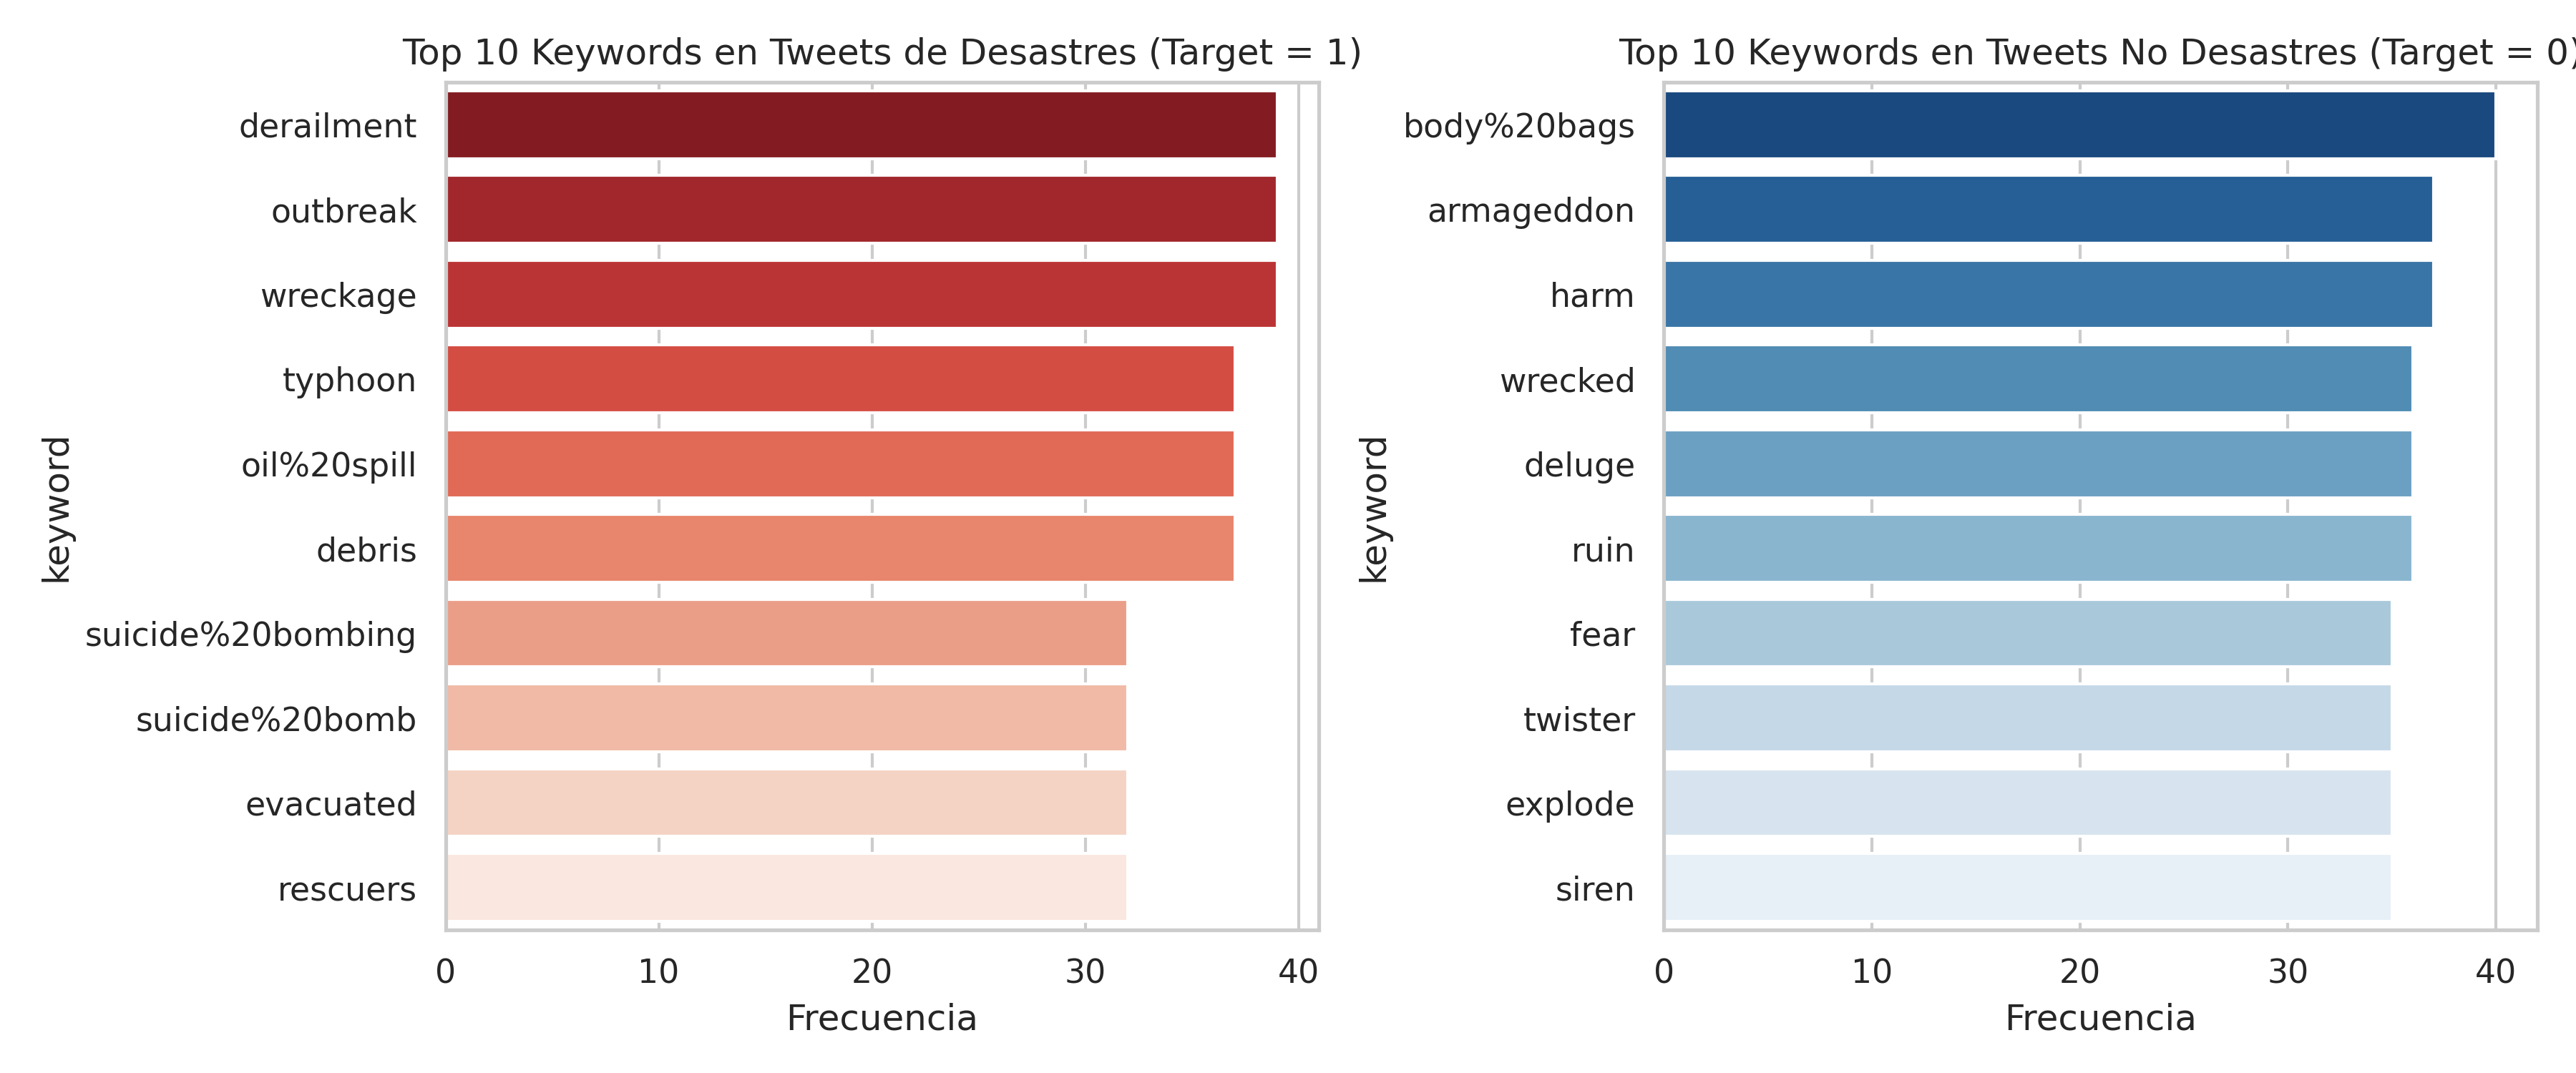
\includegraphics[width=0.9\textwidth]{figures/top_keywords.png}
    \caption{Top 10 palabras clave (\textit{keywords}) en tweets de desastres vs no desastres.}
    \label{fig:top_keywords}
\end{figure}

Asimismo, en la Figura~\ref{fig:text_length} se observa que los tweets de desastres reales tienden a poseer una mayor longitud promedio en caracteres y palabras en comparación con los tweets no relacionados a emergencias, lo cual sugiere un estilo de redacción más formal e informativo en reportes de noticias y advertencias oficiales.

\begin{figure}[H]
    \centering
    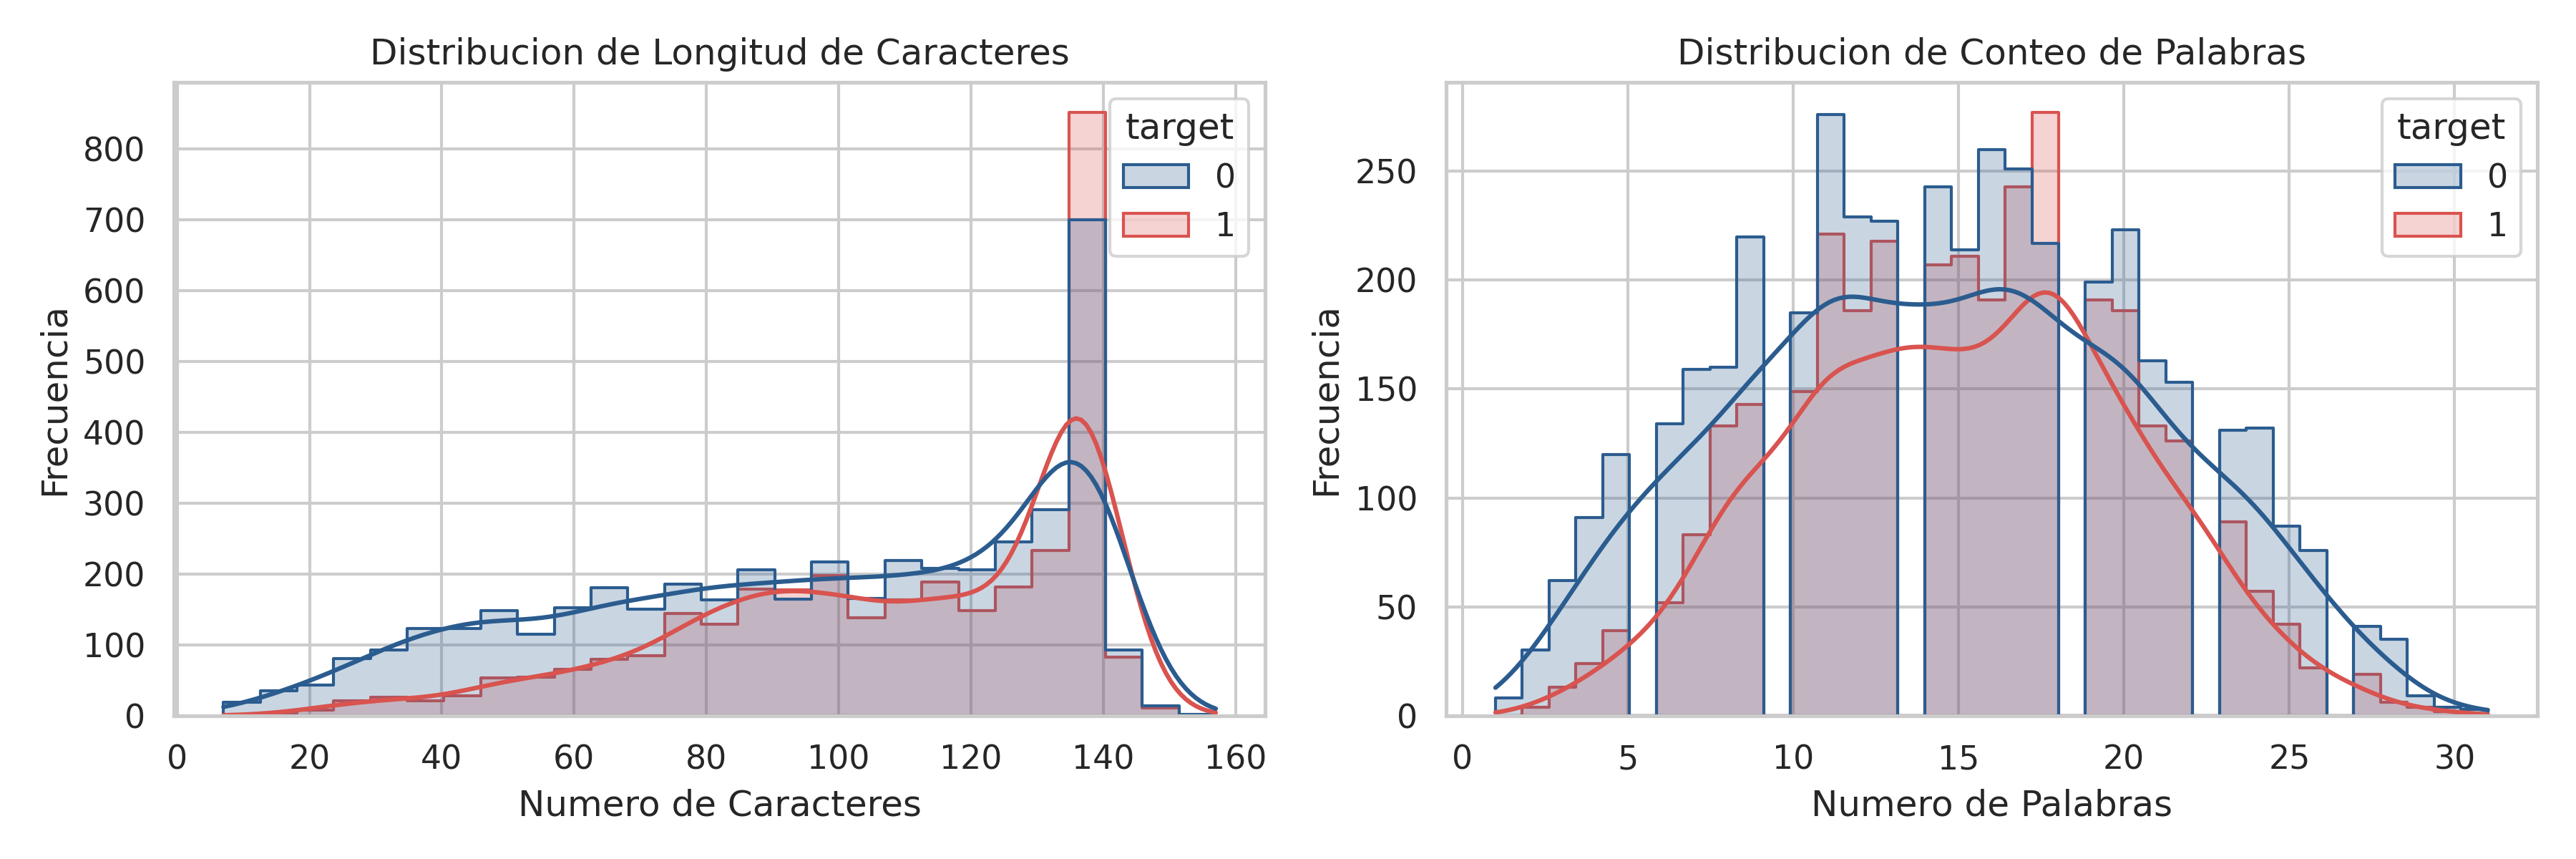
\includegraphics[width=0.9\textwidth]{figures/text_length_distribution.png}
    \caption{Distribución de la cantidad de caracteres y palabras por tweet según categoría.}
    \label{fig:text_length}
\end{figure}

\end{document}
